\subsection{Stop Words}

Stop words are typically the most commonly occurring words in text. The provided code defines a set of Bengali stop words and then removes them from a vocabulary list.

The resulting list, \textbf{wo\_stop\_words}, contains only meaningful words, excluding the common stop words. Removing stop words helps improve the efficiency of various NLP tasks by reducing the dimensionality of the data and focusing on more content-rich words, which is especially useful in tasks such as text classification, search engine optimization, and sentiment analysis.

\begin{figure}[H]
    \centering
    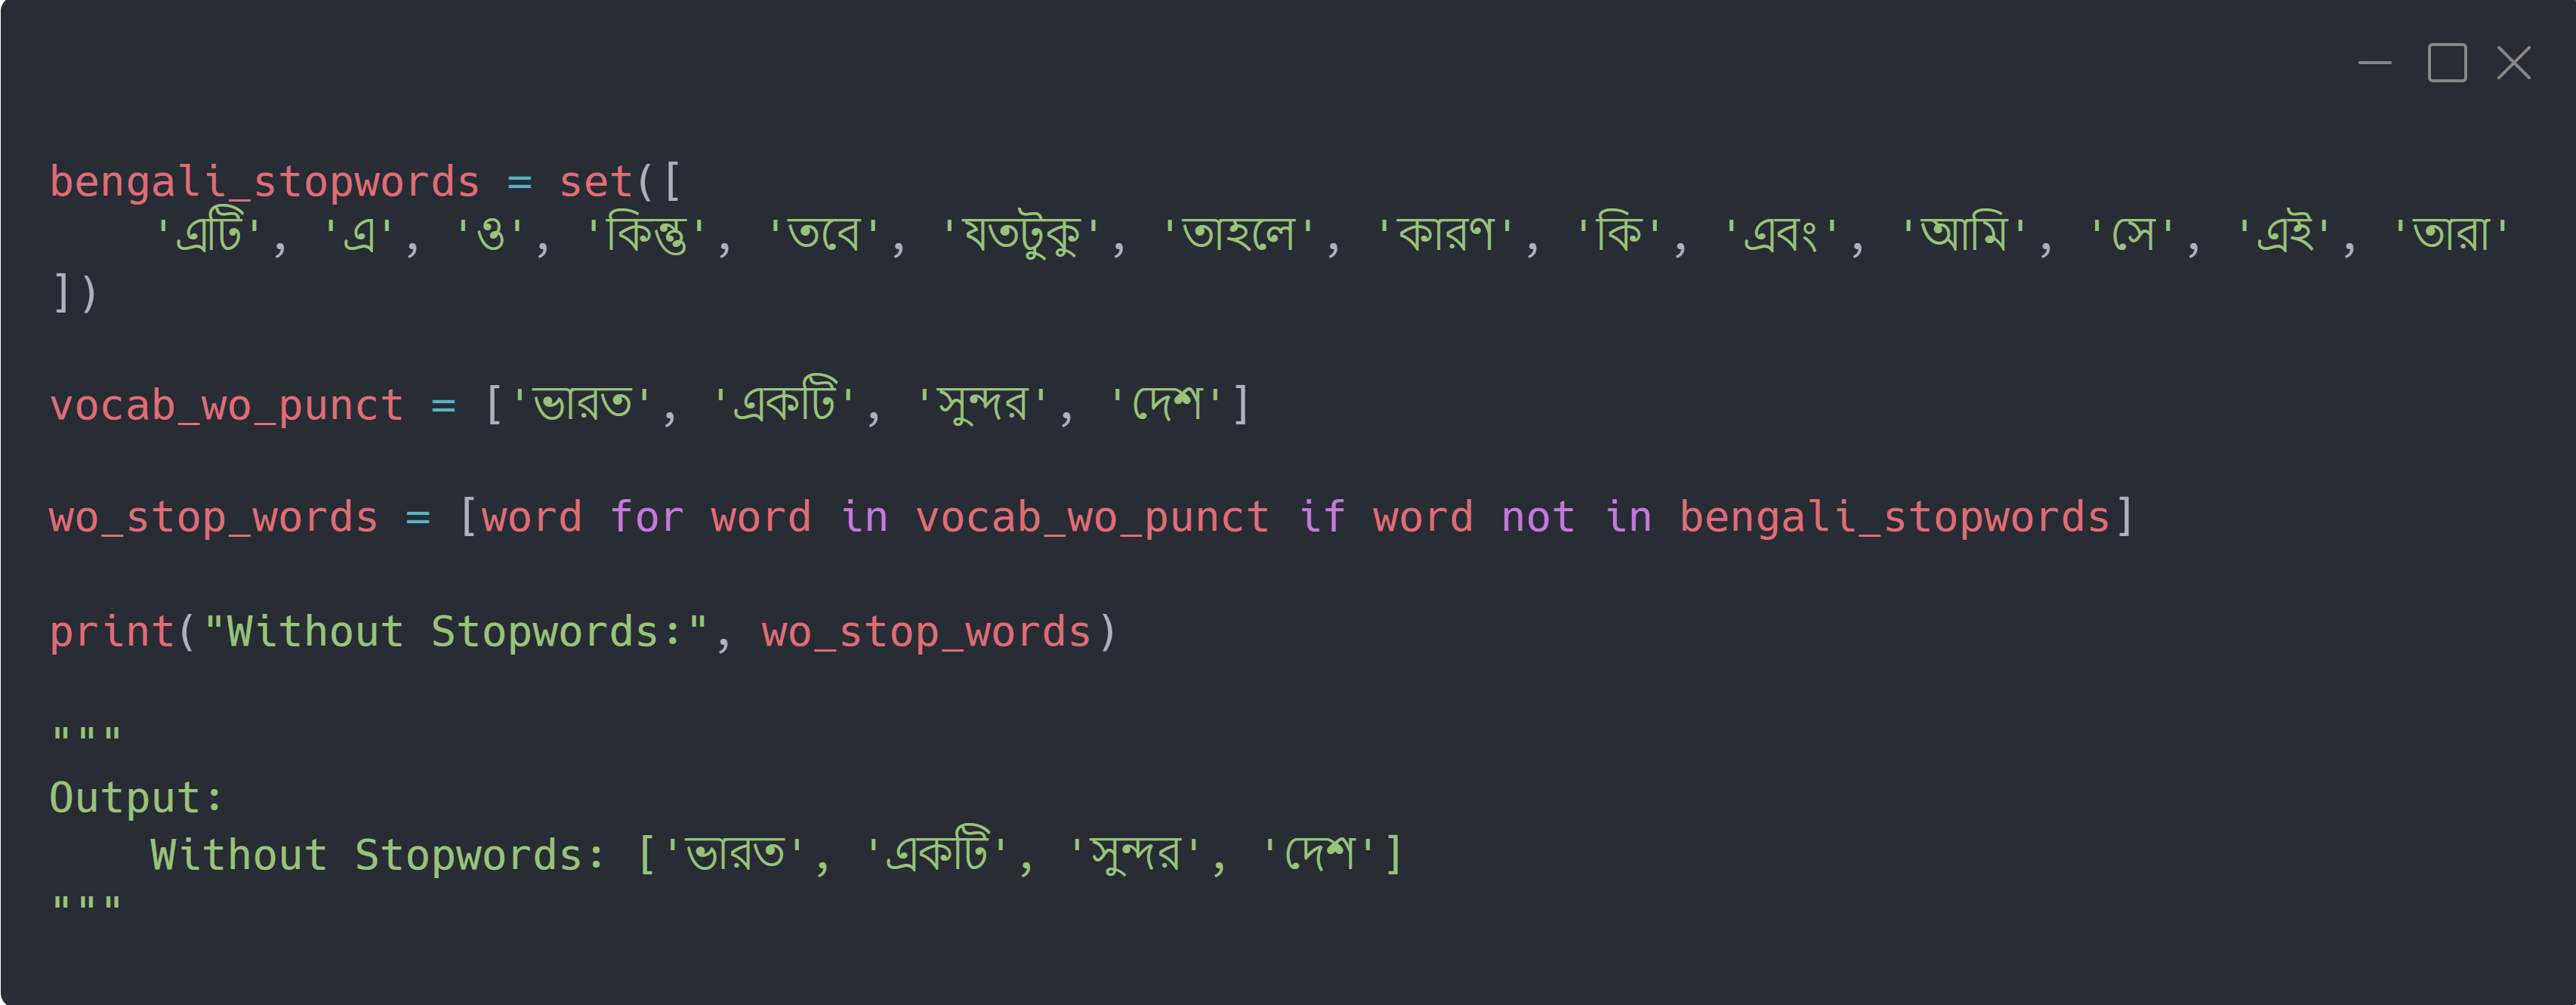
\includegraphics[width=0.8\linewidth]{Attachments/Figures/stop-words_figure1.png}
    \caption{Illustration of Stop Words removal in Bengali text.}
\end{figure}